\documentclass[9pt]{beamer}
%\usepackage[osf,sc]{mathpazo}
\usepackage{graphicx}
\usepackage{amsmath}
\usepackage{units}
\usepackage{mathtools}
\usepackage{xmpmulti}
\usepackage{animate}
\usepackage{eulervm}
\usepackage{tikz}
\usetikzlibrary{arrows,shapes,backgrounds,arrows.meta,calc}
\tikzset{%
  >={Latex[width=2mm,length=2mm]},
  % Specifications for style of nodes:
            base/.style = {rectangle, rounded corners, draw=black,
                           minimum width=35mm, minimum height=5mm,
                           text centered, font=\sffamily}
                           }
\usepackage[backend=biber,style=alphabetic,sorting=none]{biblatex}
\addbibresource{../Bibliography.bib}
\usetheme{boxes}
\usefonttheme{professionalfonts}
\usecolortheme{rose}
%\usefonttheme{serif}
\setbeamertemplate{navigation symbols}{}

\usepackage{graphicx}
\DeclareMathOperator*{\argmax}{arg\,max}
\DeclareMathOperator*{\argmin}{arg\,min}
\DeclareMathOperator*{\Var}{Var}
\DeclareMathOperator*{\COV}{Cov}

\newcommand{\expSym}{{E}}
\newcommand{\E}[1]{\ensuremath{\expSym\left(#1\right)}}
\newcommand{\prob}[1]{\ensuremath{\Pr\left(#1\right)}}
\newcommand{\T}{T}
\newcommand{\Cov}[2]{\ensuremath{\COV(#1, #2)}}
\newcommand{\bottomcite}[1]{\vspace*{\fill} {\scriptsize \parencite{#1}}}

%\renewcommand{\vec}[1]{\ensuremath{#1}}

\newcounter{multipleslide}
\makeatletter%
\newcommand{\multipleframe}{%
\setcounter{multipleslide}{\value{framenumber}}
\stepcounter{multipleslide}
\patchcmd{\beamer@@tmpl@footline}% <cmd>
  {\insertframenumber}% <search>
  {\themultipleslide}% <replace>
  {}% <success>
  {}% <failure>
}
\newcommand{\restoreframe}{%
\patchcmd{\beamer@@tmpl@footline}% <cmd>
  {\themultipleslide}% <search>
  {\insertframenumber}% <replace>
  {}% <success>
  {}% <failure>
\setcounter{framenumber}{\value{multipleslide}}%
}
\makeatother%


\usepackage{amsmath}
\usepackage{amssymb}
\usepackage{amsthm}
\usepackage{multirow}
\usepackage{mathtools}

\setbeamertemplate{footline}[frame number]

\title{Analysis of Markovian Population Models}
\subtitle{Dissertation Defense}
\author{Michael Backenk\"{o}hler}
\institute{Saarland Informatics Campus}
\date{September 20, 2022}

\begin{document}

\tikzstyle{every picture}+=[remember picture]
\tikzstyle{na} = [baseline=-.5ex]

\begin{frame}
\titlepage
\end{frame}

\begin{frame}{Motivation}
  \begin{itemize}
    \item stochastic concentration changes
    \item examples: fish and angler
    \item systems biology: switches, 
    \item applications: queueing, metabolic networks, bio-switches, traffic etc.
    \item goal: do \emph{rigorous} analysis on such models
  \end{itemize}
\end{frame}

\begin{frame}{Markovian population models}{Framework}
    \begin{columns}
        \begin{column}{.4\textwidth}
            \centering
            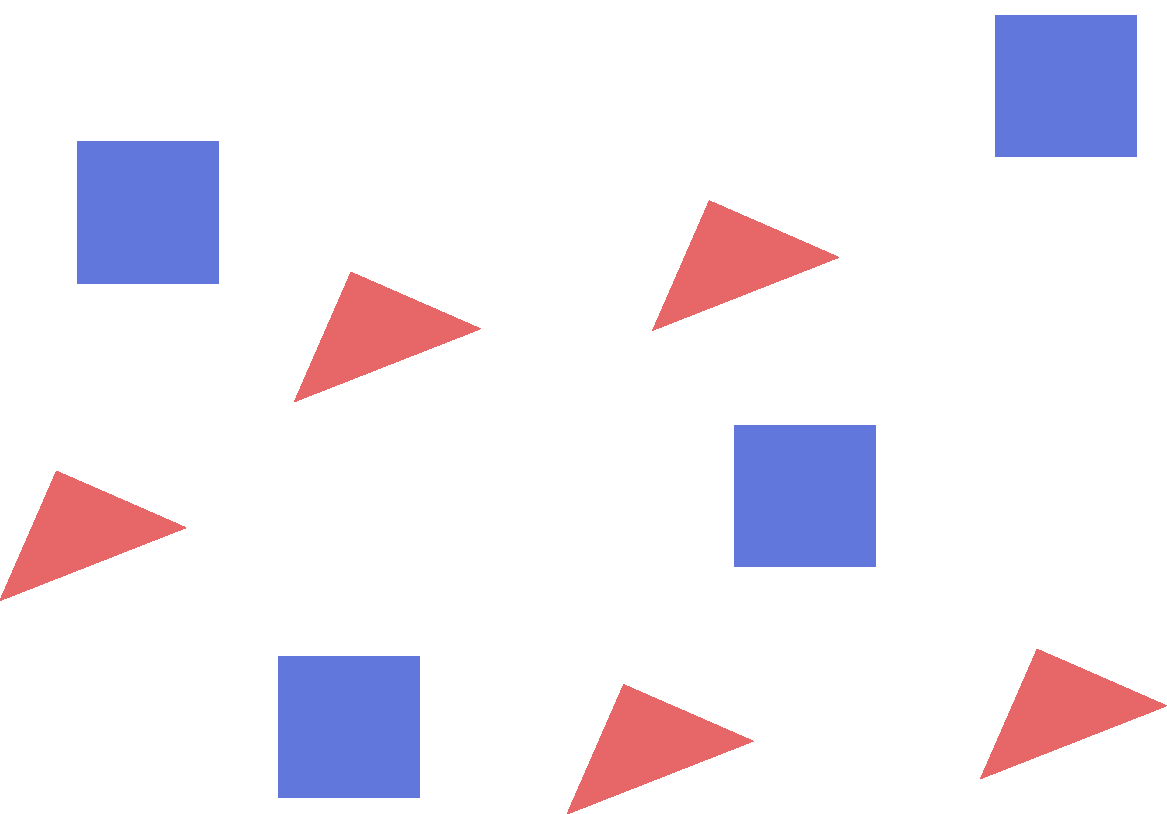
\includegraphics[width=3cm]{../gfx/populations.pdf}
            \vspace{-5mm}
            \[\underbrace{\quad\hspace{3cm}\quad}_{\textstyle (\,\underset{
\includegraphics[width=2mm]{../gfx/square.pdf}}{4}, \underset{
\includegraphics[width=3mm]{../gfx/triangle.pdf}}{5}\,)}\]
            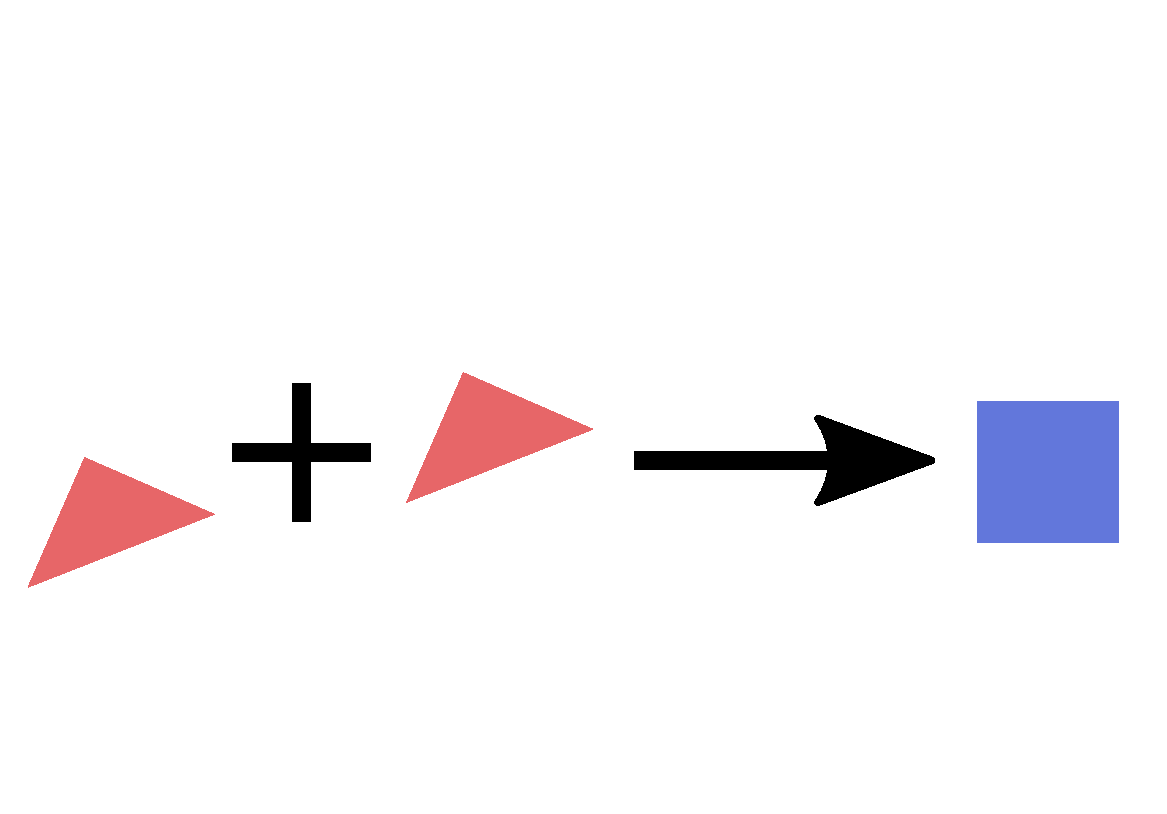
\includegraphics[width=3cm]{../gfx/reaction.pdf}
        \end{column}
        \begin{column}{.58\textwidth}
            \begin{itemize}
                \item populations of identical agents
                \item state space $\sim$ population sizes
                \item often huge to infinite
            \end{itemize}
            \vspace{1cm}
            \begin{itemize}
                \item continuous time
                \item exponential jump times / CTMC dynamics
                \item Kolmogorov equation for probabilities: \[\frac{d}{dt}\pi(t)=\pi(t)Q\]
            \end{itemize}
        \end{column}
    \end{columns}
\end{frame}

\section{Markovian population models}
\begin{frame}{Markovian population models}{How they behave}
    \begin{figure}
        \begin{exampleblock}{Example (birth-death process)}
        \begin{columns}
            \begin{column}{.05\paperwidth}\end{column}
            \begin{column}{.33\paperwidth}
                \vspace{-5mm}
                $$ {X\rightarrow \varnothing, \quad \alpha_1(x)=0.1 \cdot x } $$
                $$ {\varnothing\rightarrow X, \quad \alpha_2(x) = 10 } $$
                \vfill
            \end{column}
            \begin{column}{.6\paperwidth}
                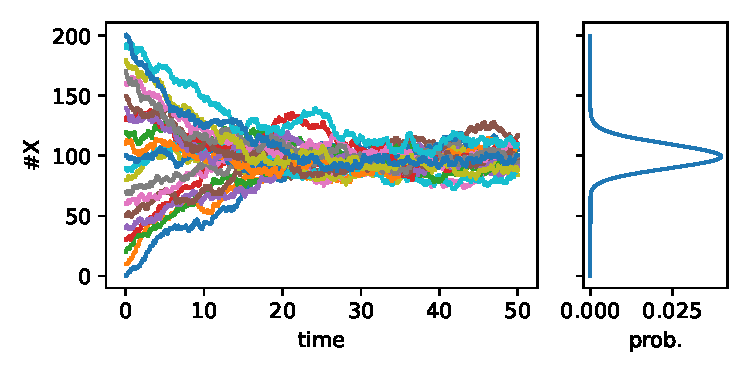
\includegraphics[width=6cm]{../gfx/stationary_dist.pdf}
            \end{column}
        \end{columns}
        \end{exampleblock}
    \end{figure}
    \begin{itemize}
        \item changes depend on current state only
        \item ergodic chains converge to unique distribution ($t\to\infty$)
        %\item problem: infinite state-spaces?
        \item Foster-Lyapunov functions for bounds
        %\item local augment functions for tighter bounds
    \end{itemize}
\end{frame}

\begin{frame}{Markovian population models}{Approaches to their analysis}
  %\begin{itemize}
    %\item expected values, e.g. $\E{X}, \E{X^2}$
    \begin{figure}
        \centering
    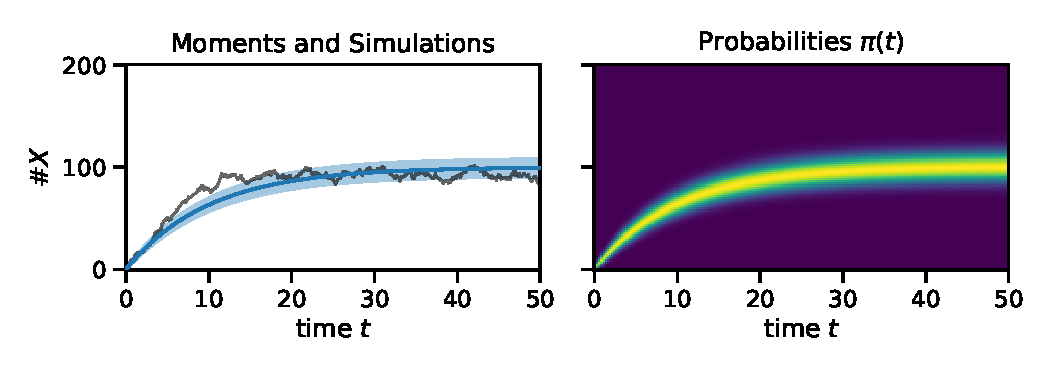
\includegraphics[scale=.45]{../gfx/momsandprobs.pdf}
    \end{figure}
          \begin{block}{Moment equation}
              Moments such as mean $\E{X_t}$ and variance $\E{X_t^2}-\E{X_t}^2$ are described by (often {linear}) ODEs.
        \begin{equation*}
            \frac{d}{dt}\E{f({\vec{ X}}_t)} = \sum_{j=1}^{n_R}\E{\left(f({\vec X_t +
            \vec{v}_j}) - f(\vec X_t)\right)\alpha_j(\vec X_t)}
        \end{equation*}
          \end{block}
    %\item ODE system usually not closed
  %\end{itemize}
\end{frame}
% typically closed by MC, but can be forgone if not integration is desired

\section{Moment-based Methods}
\begin{frame}
  \vfill
  \centering
    \usebeamerfont{title}\insertsectionhead\par%
    \vspace{1cm}
    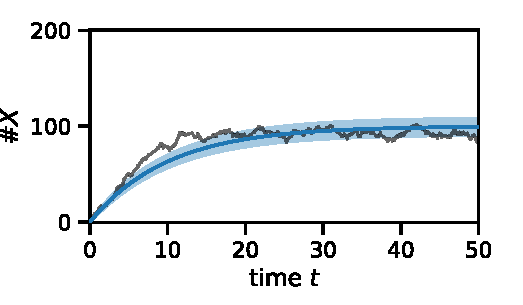
\includegraphics[width=5cm]{../gfx/momsandsims.pdf}
  \vfill
\end{frame}

\begin{frame}{Markovian population models}{Martingale process}
    \begin{itemize}
        \item start with the moment ODE
    \item multiply time-weighting: $w(t)=t^k$, $k\in\mathbb{N}$ or $w(t)=\exp(\lambda t)$
    \item analytic integration results in a martingale 
        \begin{equation*}
            \begin{split}
            Z_T\coloneqq&\,w(T)f(\vec X_T) - w(0)f(\vec X_{0}) -
            \int_{0}^T\frac{dw(t)}{dt}f(\vec X_t)\,dt\\
            &-\sum_{j=1}^{n_R}\int_{0}^Tw(t)
                 (f(\vec X_t+\vec v_j) - f(\vec X_t))\alpha_j(\vec X_t)\,dt
         \end{split}
        \end{equation*}
    \item known expectation: $\E{Z_T}=0$, $\forall T\geq 0$
  \end{itemize}
    \begin{example}
    \vspace{-1em}
    \begin{figure}
        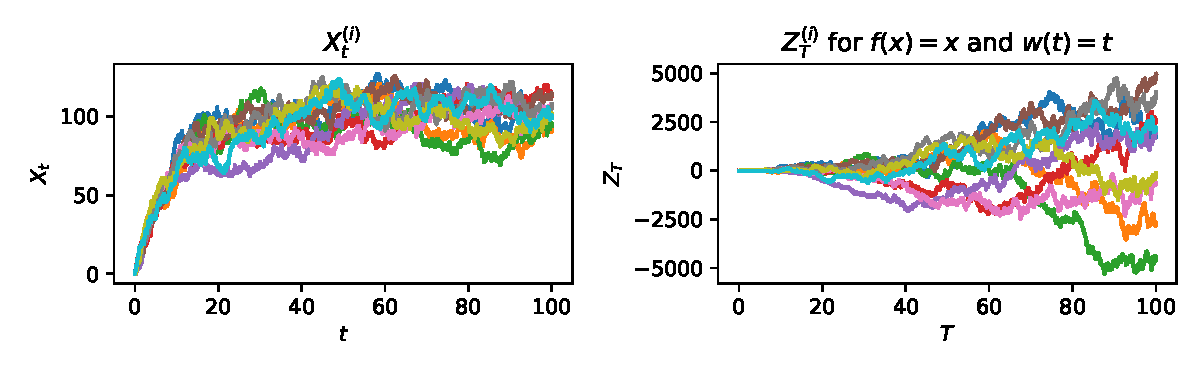
\includegraphics[scale=.5]{../gfx/martingales.pdf}
    \end{figure}
    \vspace{-1em}
    \end{example}
\end{frame}

\section{Bounding mean first-passage times}
\begin{frame}{Bounding mean first-passage times}{Linear moment constraints}
    \begin{columns}
        \begin{column}{.4\paperwidth}
            \vspace{5mm}
            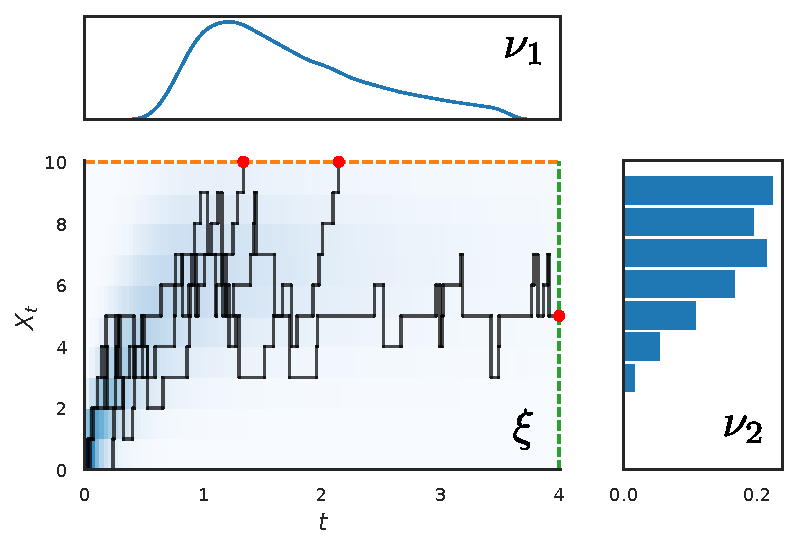
\includegraphics[scale=.4]{../gfx/decomp1.pdf}
        \end{column}
        \begin{column}{.45\paperwidth}
            \begin{itemize}
                \item $\tau=\inf\{X_t \geq H \mid t\geq 0\}\land T$
                \item time weighting $w(t)=t^k$
                \item exp.\ occupation measure $\xi$
                \item exit location measures $\nu_1$, $\nu_2$
            \end{itemize}
        \end{column}
    \end{columns}

    \begin{block}{Linear moment constraint}
        \vspace{-3mm}
\begin{multline*}\label{eq:model_constraints}
    0 = \E{Z_T} = T^k\overbrace{\E{X_{\tau}^m;\tau=T}}^{\nu_1} + H^m\overbrace{\E{{\tau}^k;\tau < T, X_{\tau}=H}}^{\nu_2}\\
 	- 0^kx_0^{m}
 	% - k \E{\int_{0}^{\tau} t^{k-1} \vec X_t^m\,dt}
    + \sum_{i}c_i\underbrace{\E{\int_{0}^{\tau} t^{k_i}X_t^{m_i}\,dt}}_{\xi}
\end{multline*}
    \end{block}
    %\begin{itemize}
        %\item $0=\E{ Z_T }$ is a linear moment constraint constraint on $\nu_1$, $\nu_2$, and $\xi$ ($w(t)=t^k$) (TODO: integrate moms and figure)
    %\end{itemize}
\bottomcite{backenkohler2019bounding}
\end{frame}

\begin{frame}{Bounding mean first-passage times}{Moment matrices}
  %\begin{itemize}
    %\item semi-definite moment constraints (positive variance as example)
    %\item hint at localizing matrices
  %\end{itemize}
    \begin{block}{Moment matrices}
    The \emph{moment matrix} must be \emph{positive semi-definite}.
    \[
        \E{\begin{matrix}
            X^0 & X^1 & X^2 & \dots & X^n \\
            X^1 & X^2 & \ddots & \ddots & \vdots \\
            \vdots & \ddots & \ddots & \ddots & \vdots \\
            X^n & X^{n+1} & \dots & \dots & X^{2n}
        \end{matrix}}\succeq 0 \,,
    \]
        where $M\succeq 0$ iff.\ $\forall v \in \mathbb{R}^n. v^T M v\geq 0$.
    \end{block}
          \begin{exampleblock}{Example}
              Let
              $M=\left(\begin{matrix} 1 & \E{X} \\
              \E{X} & \E{X^2} \end{matrix}\right)$. Then $\det M = \E{X^2}-\E{X}^2 = \sigma^2 \geq 0$.
%By \emph{Sylvester's criterion} $M\succeq 0$ iff.\ $\det M \geq 0$. Clearly, $\det M = \E{X^2}-\E{X}^2 = \sigma^2 \geq 0$.
          \end{exampleblock}
\bottomcite{backenkohler2019bounding}
\end{frame}

\begin{frame}{Bounding mean first-passage times}{Semi-definite program}
  \begin{itemize}
    \item measure support can be restricted using semi-definite constraints
    \item resulting SDPs can be solved using off-the-shelf software.
    \begin{block}{Semi-definite program (SDP)}
        An optimization problem with
        \begin{enumerate}
            \item \emph{linear constraints} on moments and
            \item \emph{positive semi-definite constraints} on certain matrices.
        \end{enumerate}
    \end{block}
    \item alternative: linear \emph{Hausdorff constraints} instead of semi-definite constraints
        \[\int_{[0,1]^{\vec n}}{\vec x}^{\vec\ell}{(1-\vec x)}^{\vec k}\,d\mu(\vec x)\geq 0\]
  %\begin{itemize}
    %\item linear constraints possible if domains (time and space) are finite
    %\item 1D visualization of Hausdorff constraints
  %\end{itemize}
  \end{itemize}
\bottomcite{backenkohler2019bounding}
\end{frame}

\begin{frame}{Bounding mean first-passage times}{Results}
    \begin{columns}
        \begin{column}{.33\paperwidth}
            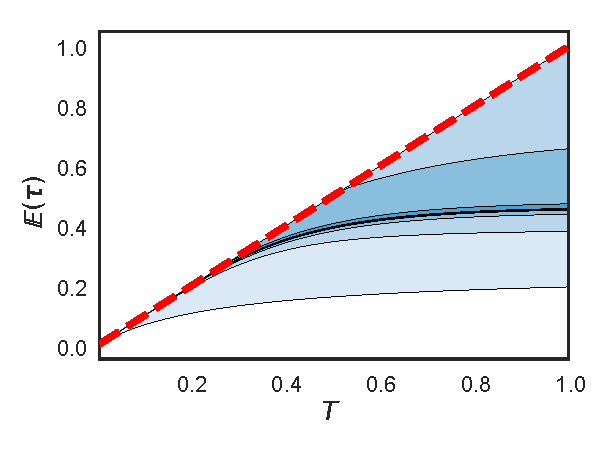
\includegraphics[width=\textwidth]{../gfx/mfpt_bounds.pdf}
        \end{column}
        \begin{column}{.57\paperwidth}
            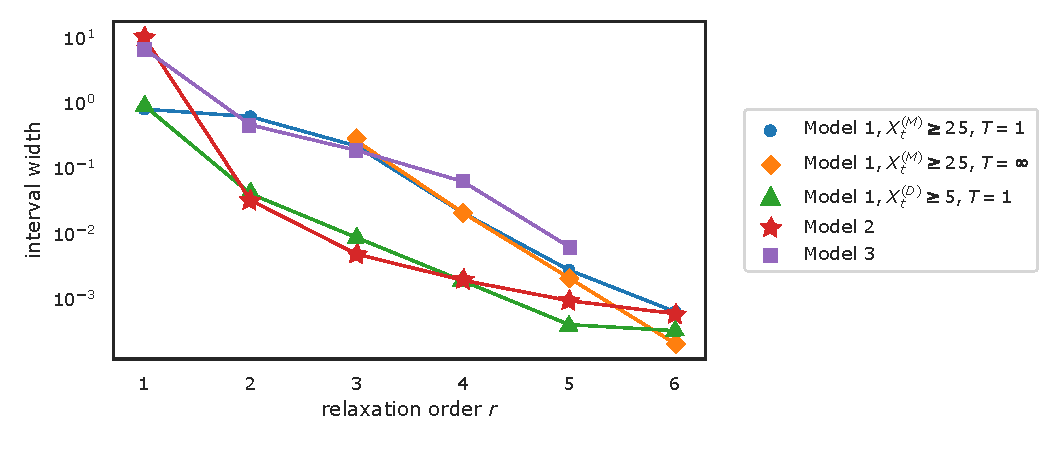
\includegraphics[width=\textwidth]{../gfx/convergence.pdf}
        \end{column}
    \end{columns}
    \vspace{2em}
    \begin{itemize}
        \item fast convergence of bounds with increasing order
        \item SDPs are usually solved within seconds
        \item numerically challenging (inherent stiffness)
        \item scaling state-space / model size is difficult
    \end{itemize}
\bottomcite{backenkohler2019bounding}
\end{frame}

\section{Linear control variates}
\begin{frame}{Linear control variates}{Using correlated RVs with known expected value}
    \begin{columns}
        \begin{column}{.03\paperwidth}
        \end{column}
        \begin{column}{.4\textwidth}
            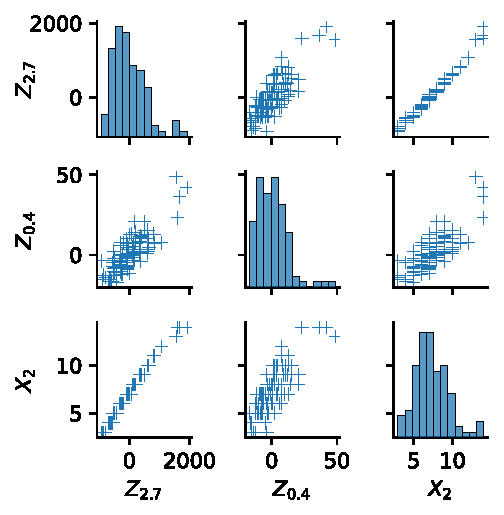
\includegraphics[width=.8\textwidth]{../gfx/correlation.pdf}
        \end{column}
        \begin{column}{.50\paperwidth}
            \begin{itemize}
                \item improve MC estimates using $Z_T$
                \item use correlations between $Z_T$ and $X_T$
                \item $\E{X_T + b Z_T}$ instead of $\E{X_T}$\\ (recall $\E{Z_T}=0$)
                \item time-weighting $w(t)=\exp(\lambda t)$
            \end{itemize}
        \end{column}
    \end{columns}
    \begin{block}{Linear control variates}
        \begin{columns}
            %\begin{column}{.01\textwidth}
            %\end{column}
            \begin{column}{.6\textwidth}
                Given a control variate vector $\vec{Z}$, the estimator
                \[\hat{V} -({\hat\Sigma_{ \vec{Z}}}^{-1}{\hat\Sigma}_{ \vec{Z} V})^{\T}{\hat{\vec{Z}}} \]
                has lower or equal variance as $\hat{V}$.
            \end{column}
            \begin{column}{.2\textwidth}
                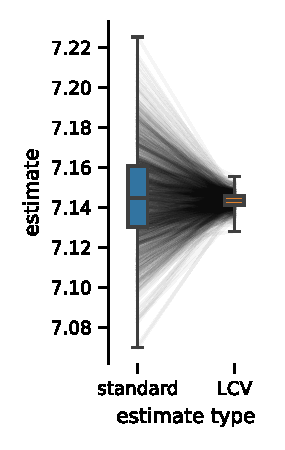
\includegraphics[width=20mm]{../gfx/adjustment_trans.pdf}
            \end{column}
        \end{columns}
    \end{block}
    \bottomcite{backenkohler2019control}
\end{frame}

\begin{frame}{Linear control variates}{Efficiency trade-off}
    \begin{itemize}
        \item infinite possible $Z$
        \item different time-weighting $\lambda$ $\rightarrow$ different correlation
        \item the trade-off:
    \begin{columns}
        \begin{column}{.5\textwidth}
            \begin{block}{cost: slowdown}
                \vspace{1ex}
                \begin{center}
                    \scalebox{1.7}{$ \nicefrac{{\text{cost}}_{\text{old}}}{{\text{cost}}_{\text{new}}} $}
                \end{center}
                \begin{itemize}
                    \item computing $\int_{0}^T w(t)X_t^m\,dt$
                    \item computing the estimate
                \end{itemize}
            \end{block}
        \end{column}
        \begin{column}{.5\textwidth}
            \begin{block}{benefit: variance reduction}
                \vspace{1ex}
                \begin{center}
                    \scalebox{1.7}{$ \nicefrac{\sigma^2_{\text{new}}}{\sigma^2_{\text{old}}} $}
                \end{center}
                \begin{itemize}
                    \item highly correlated variates
                \end{itemize}
            \end{block}
        \end{column}
    \end{columns}
            \vspace{1em}
    \item approach: correlations between candidates and the target RV
    \end{itemize}
            %\[
%\begin{bmatrix}
%1 & \dots & \rho_{1k} & \rho_{1v} \\
%\vdots & \ddots & \vdots & \vdots \\
%\rho_{k1} & \dots & 1 & \rho_{kv} \\
%\rho_{v1} & \dots & \rho_{vk} & 1
%\end{bmatrix}\,.
        %\]
  %\begin{itemize}
    %\item time-weighting has a large influence on the correlation
    %\item Infinitely many possibilities (cost needs to be controlled though)
    %\item variates can be highly redundant (correlated) and incur an additional cost
    %\item Alg.~1: Tighten an initial proposal set
    %\item Alg.~2: Re-sample promising candidates
  %\end{itemize}
    \bottomcite{backenkohler2019control,backenkohler2021variance}
\end{frame}

\begin{frame}{Linear control variates}{Selection by filtering}
    \begin{columns}
       \begin{column}{.4\textwidth}
            \begin{block}{Algorithm 1}
                \begin{figure}
                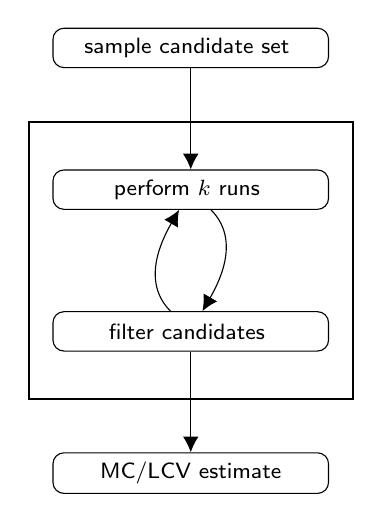
\begin{tikzpicture}[node distance=1.8cm,
                every node/.style={fill=white, font=\sffamily}, align=center]
                    \node (initial) [base]                    {\footnotesize  sample candidate set };
                    \node (pilot)   [base, below of=initial]  {\footnotesize  perform $k$ runs };
                    \node (filter)  [base, below of=pilot]    {\footnotesize  filter candidates };
                    \node (mc)      [base, below of=filter]   {\footnotesize  MC/LCV estimate};

                    \draw[->]  (initial) -- (pilot);
                    \draw[->]  (pilot)   to[out=315, in=60] (filter);
                    \draw[->]  (filter)  to[out=135, in=240] (pilot);
                    \draw[->]  (filter)  -- (mc);

                    \draw[thick] ($(pilot.north west)+(-0.3,0.6)$)  rectangle ($(filter.south east)+(0.3,-0.6)$);

                    %\node (label) [above of=pilot, xshift=.2, yshift=.5] { $k$ iterations };
                \end{tikzpicture}
                \end{figure}
            \end{block}
        \end{column}
        \begin{column}{.55\textwidth}
            filter criteria:
            \begin{enumerate}
                \item low target correlation
                    %\[ \rho_{iv} < \max \left(0.1, \frac{\max_j \rho_{jv}}{k_{\min}}\right) \]
                \item various redundancy heuristics
                    %criteria based on $\rho_{ij}$ and $\rho_{iv}$
            \end{enumerate}
            \vspace{2em}
                    \begin{columns}
                        %\begin{column}{.6\textwidth}
                            %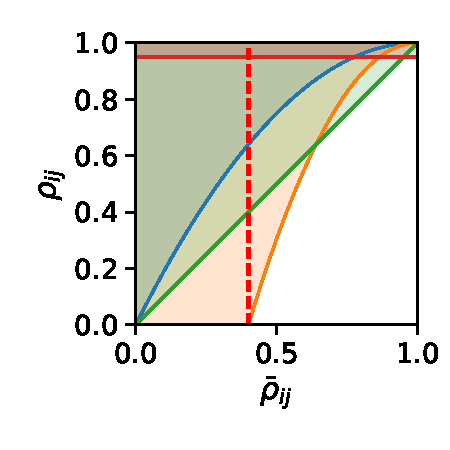
\includegraphics[width=\textwidth]{../gfx/decision_funcs.pdf}
                        %\end{column}
                        %\begin{column}{.39\textwidth}
                            %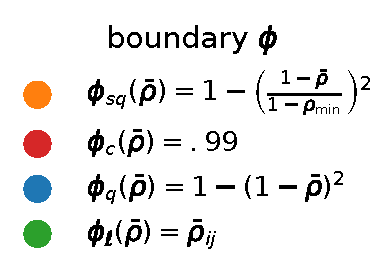
\includegraphics[width=\textwidth]{../gfx/legend_1.pdf}
                        %\end{column}
                        \begin{column}{.6\textwidth}
                            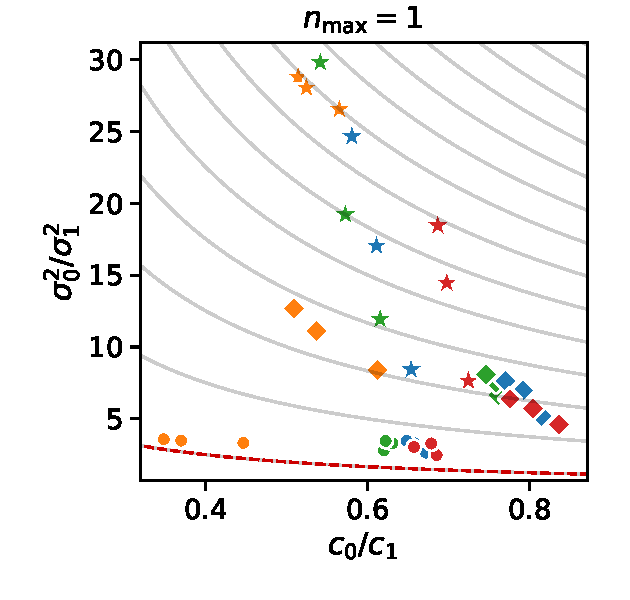
\includegraphics[width=\textwidth]{../gfx/eff_landscape_order1.pdf}\\
                        \end{column}
                        \begin{column}{.39\textwidth}
                            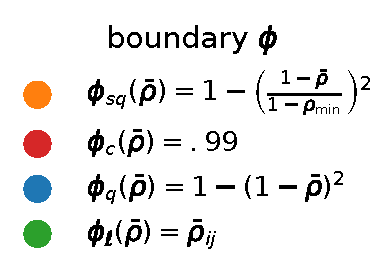
\includegraphics[width=\textwidth]{../gfx/legend_1.pdf}
                            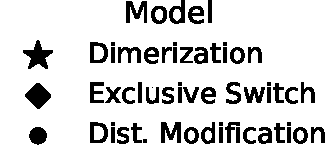
\includegraphics[width=\textwidth]{../gfx/legend_models.pdf}
                        \end{column}
                    \end{columns}
        \end{column}
    \end{columns}
    \bottomcite{backenkohler2019control}
\end{frame}
% less choices to be made; 1 parameter for selection part
\begin{frame}{Linear control variates}{Selection by resampling}
    \begin{columns}
       \begin{column}{.4\textwidth}
            \begin{block}{Algorithm 2}
                \begin{figure}
                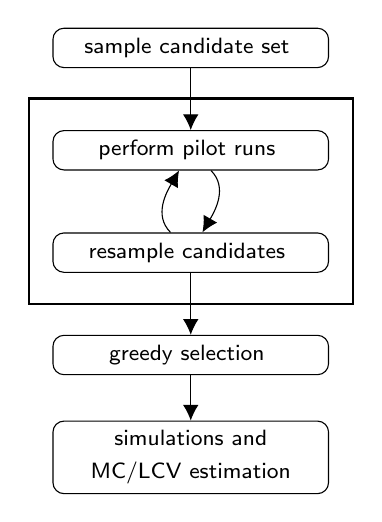
\begin{tikzpicture}[node distance=1.3cm,
                every node/.style={fill=white, font=\sffamily}, align=center]
                    \node (initial) [base]                    {\footnotesize  sample candidate set };
                    \node (pilot)   [base, below of=initial]  {\footnotesize  perform pilot runs };
                    \node (filter)  [base, below of=pilot]    {\footnotesize  resample candidates };
                    \node (greedy)  [base, below of=filter]   {\footnotesize  greedy selection };
                    \node (mc)      [base, below of=greedy]   {\footnotesize  simulations and\\ \footnotesize MC/LCV estimation};

                    \draw[->]  (initial) -- (pilot);
                    \draw[->]  (pilot)   to[out=315, in=60]  (filter);
                    \draw[->]  (filter)  to[out=135, in=240] (pilot);
                    \draw[->]  (filter)  -- (greedy);
                    \draw[->]  (greedy)  -- (mc);

                    \draw[thick] ($(pilot.north west)+(-0.3,0.4)$)  rectangle ($(filter.south east)+(0.3,-0.4)$);

                    %\node (label) [above of=pilot, xshift=.2, yshift=.5] { $k$ iterations };
                \end{tikzpicture}
                \end{figure}
            \end{block}
        \end{column}
        \begin{column}{.55\textwidth}
            \begin{itemize}
                \item \emph{resampling}: proportional to improvement % explained variance
                    %\[ \gamma_{kv} = (1 - \rho_{kv}^2)^{-1} \]
                    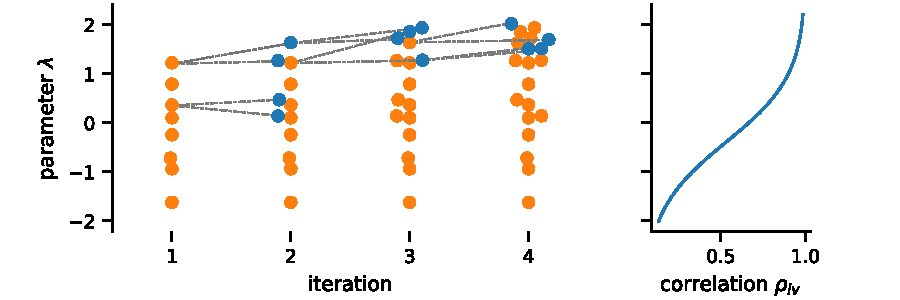
\includegraphics[width=\textwidth]{../gfx/resampling.pdf}
                \item \emph{selection}: greedy by improvement% of one CV
                    %\[
%\argmax_{1\leq i \leq \left|P_{\text{all}}\right|}
%\hat{\gamma}_{iv}
    %\prod_{\substack{1\leq j\leq {\left|P_{\text{all}}\right|}\\(m_j, \lambda_j)\in P^*}}
    %\hat{\gamma}_{ij}^{-1}
%\]
            \end{itemize}
            \vspace{2em}
            \noindent
            Results:
            \begin{itemize}
                \item performance equal/better than Alg.~1
                \item less hyper-parameter headaches
            \end{itemize}
        \end{column}
    \end{columns}
    \bottomcite{backenkohler2021variance}
\end{frame}
\section{Aggregation {\&} refinement}
\begin{frame}
      \vfill
  \centering
    \usebeamerfont{title}\insertsectionhead\par%
    \vspace{1cm}
    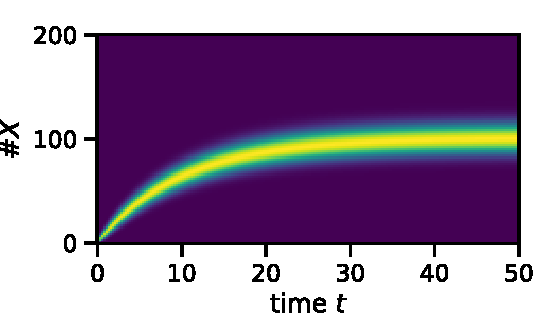
\includegraphics[width=5cm]{../gfx/bd_dist.pdf}
  \vfill
\end{frame}

\begin{frame}{State-space truncation}
    \begin{columns}
        \begin{column}{.30\textwidth}
            \begin{block}{Original}
                \centering
                \vspace{3mm}
                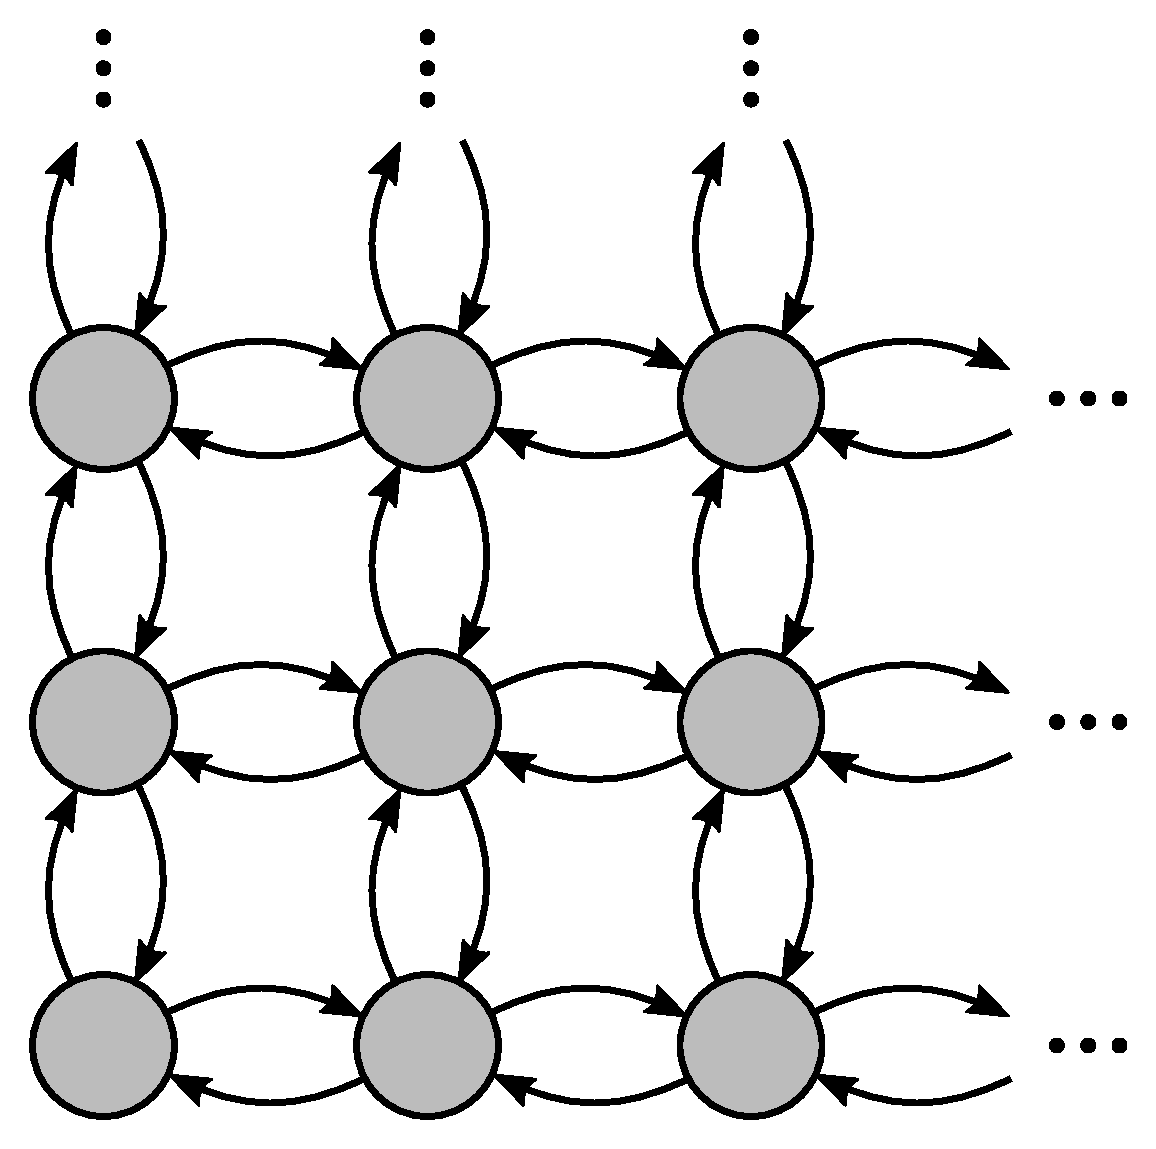
\includegraphics[height=2cm]{../gfx/state_space_untrunc.pdf}
                {\small
                \begin{itemize}
                    \item very large/infinite
                    \item impossible to analyze
                \end{itemize}
                }
            \end{block}
        \end{column}
        \begin{column}{.30\textwidth}
            \begin{block}{Sink state}
                \centering
                \vspace{3mm}
                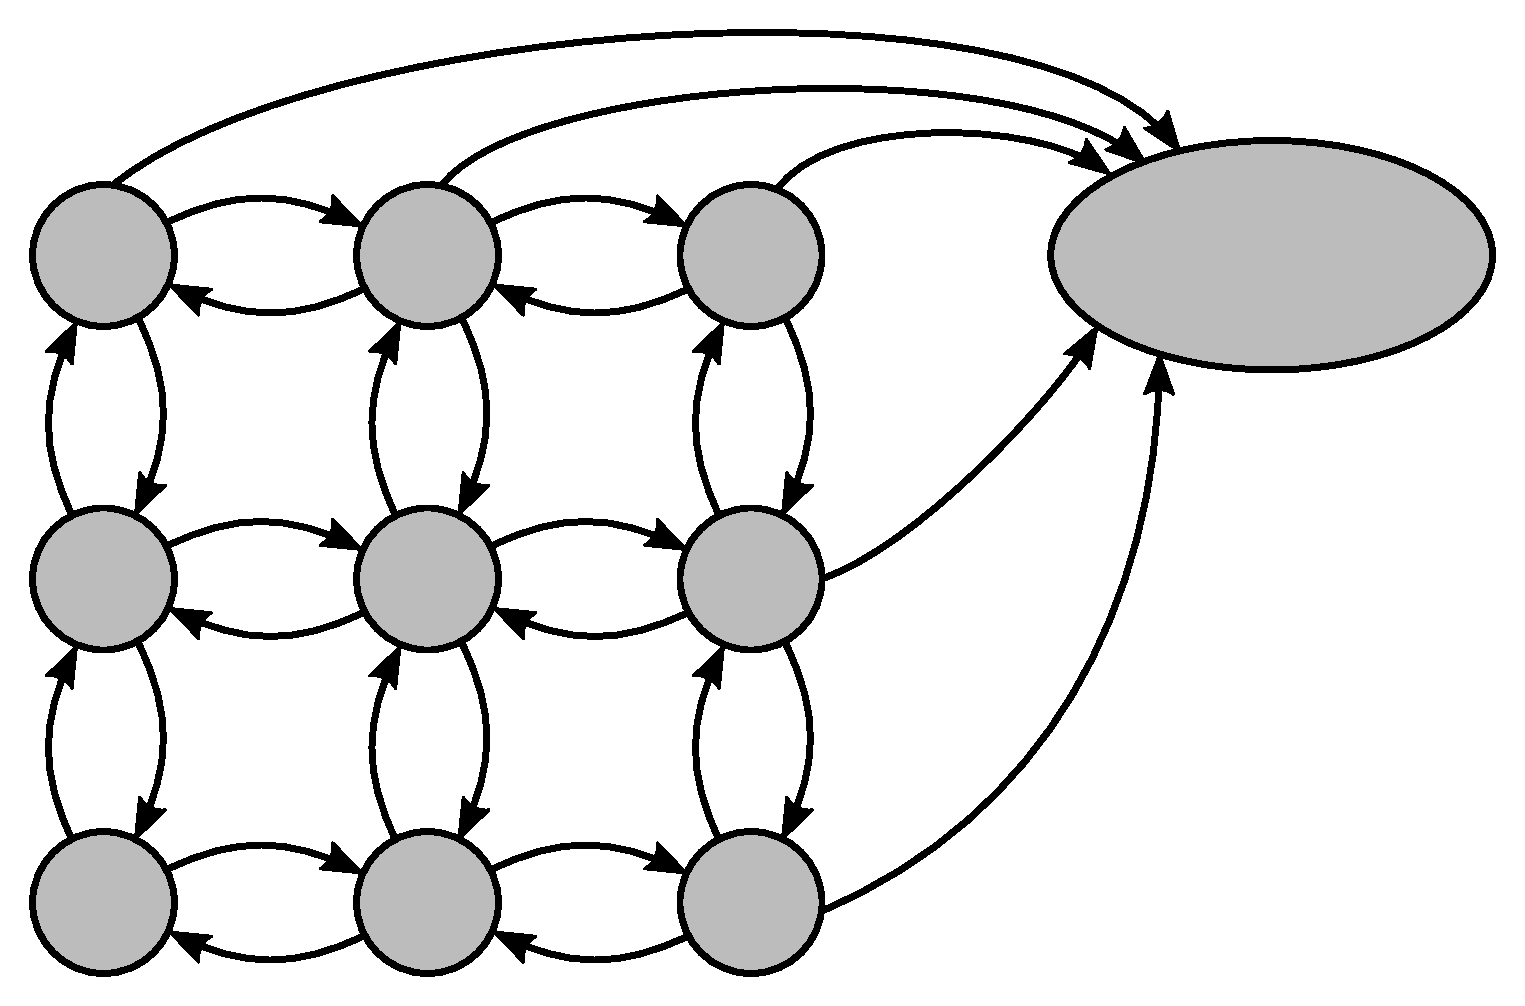
\includegraphics[height=2cm]{../gfx/state_space_redirected.pdf}
                {\small
                \begin{itemize}
                    \item transient analysis
                    \item keep track of approx.\ error
                \end{itemize}
                }
            \end{block}
        \end{column}
        \begin{column}{.30\textwidth}
            \begin{block}{Redirection}
                \centering
                \vspace{3mm}
                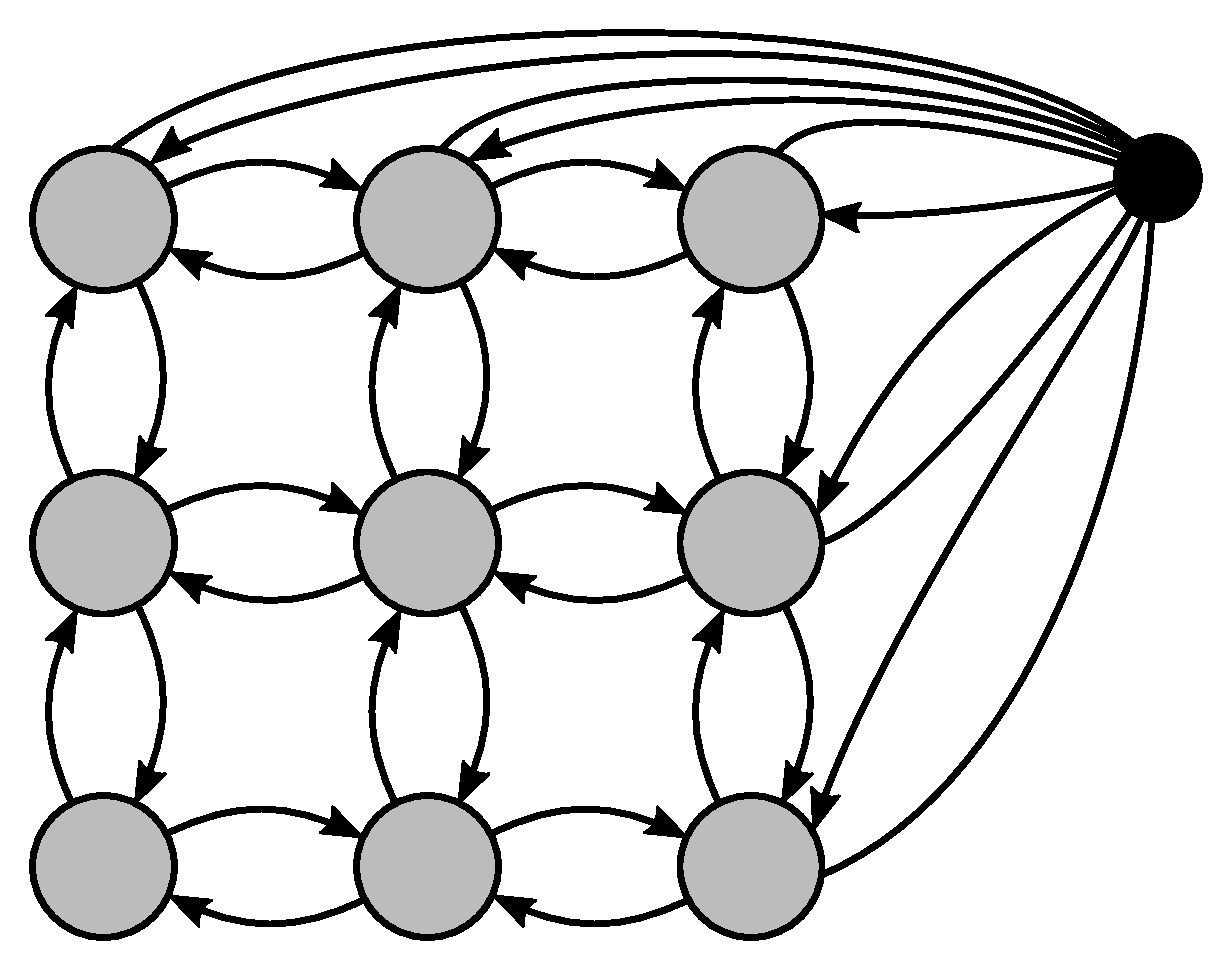
\includegraphics[height=2cm]{../gfx/state_space_reentry.pdf}
                {\small
                \begin{itemize}
                    \item stationary dist.
                    \item dependent on redirection
                \end{itemize}
                }
            \end{block}
        \end{column}
    \end{columns}
\end{frame}

\begin{frame}{State-space aggregation}{Treating hyper-cubes of states as one}
    \begin{columns}
        \begin{column}{.4\textwidth}
            \begin{figure}
            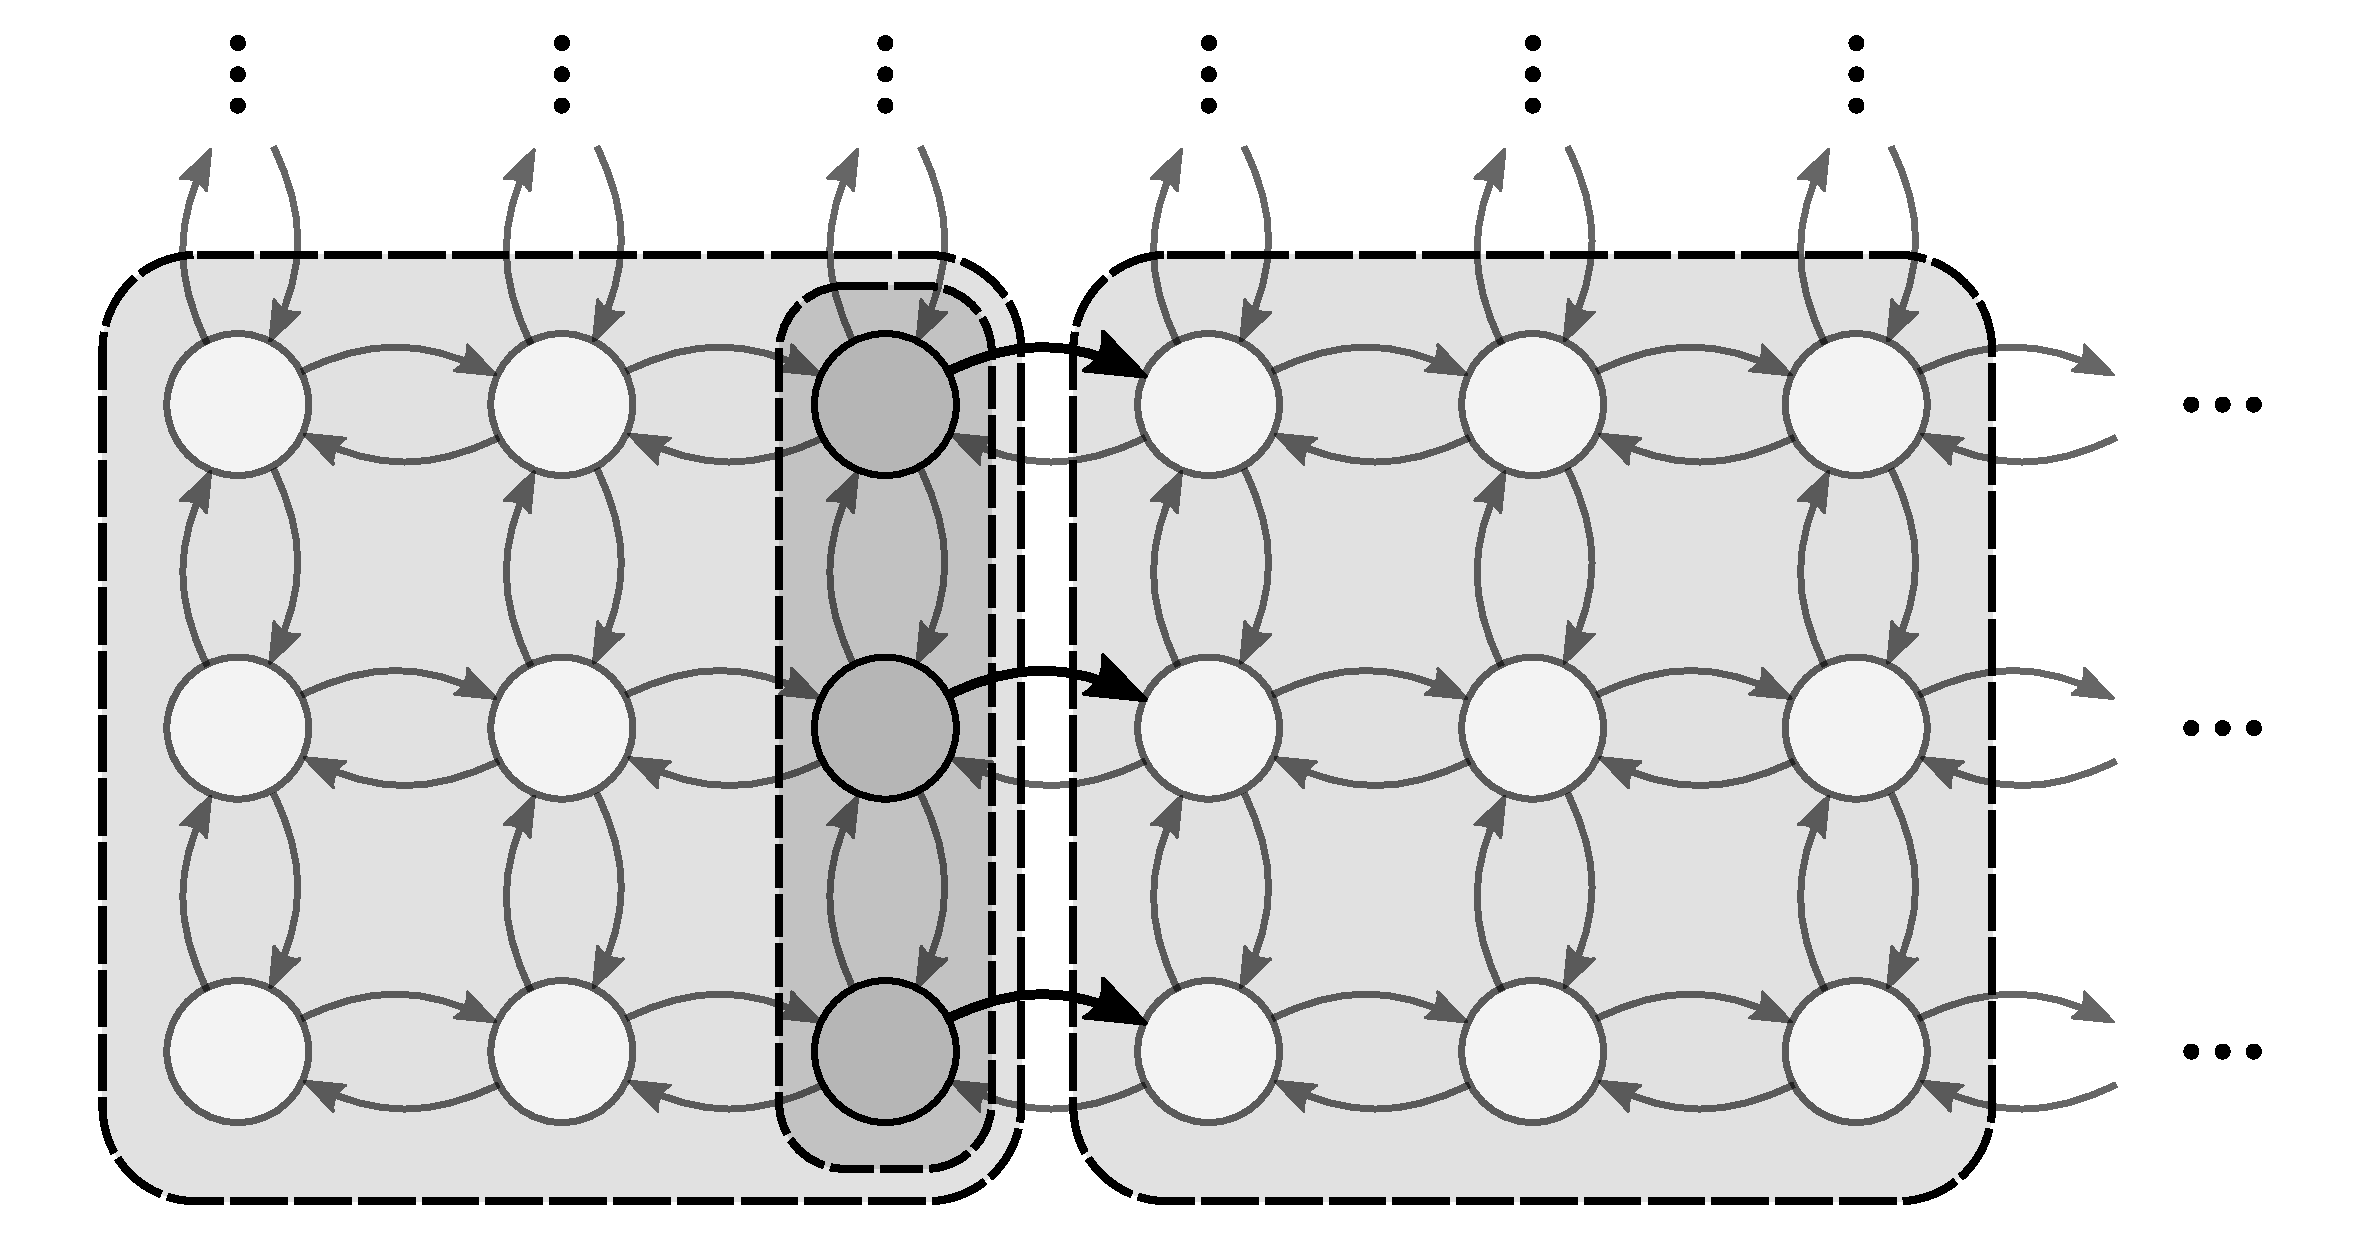
\includegraphics[width=5cm]{../gfx/macro_states.pdf}
            \end{figure}
        \end{column}
        \begin{column}{.6\textwidth}
            \begin{itemize}
                \item hyper-cube macro-states
                \item \emph{assumption}: uniform dist.\ within
                \item closed-form transition rates
            \end{itemize}
        \end{column}
    \end{columns}
    \vspace{3mm}
    \begin{exampleblock}{Example (birth-death process)}
        \begin{columns}
            \begin{column}{.4\textwidth}
                \vspace{-2em}
                \begin{figure}
                    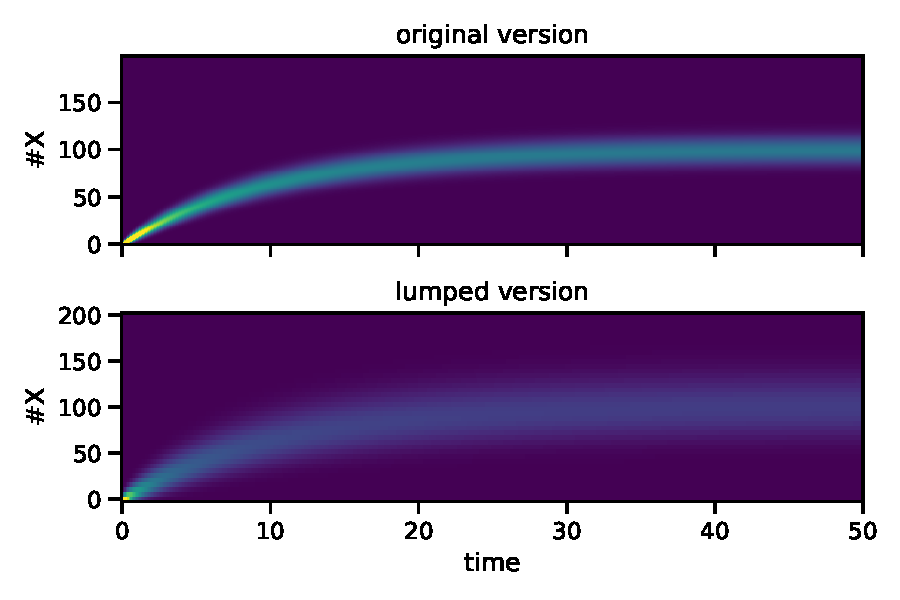
\includegraphics[width=50mm]{../gfx/lumpedvorig.pdf}
                \end{figure}
            \end{column}
            \begin{column}{.5\textwidth}
                \begin{itemize}
                    \item resulting distribution more ``flat''
                    \item  main probability masses coincide
                \end{itemize}
            \end{column}
        \end{columns}
    \end{exampleblock}
    \bottomcite{backenkohler2021abstraction}
\end{frame}

\begin{frame}{Stationary distribution}{Iterative refinement algorithm}
    \begin{columns}
        \begin{column}{.1\paperwidth}
        \end{column}
        \begin{column}{.85\paperwidth}
    A simple refinement based on approximate solutions:
    \begin{enumerate}
        \item start with macro-states of size $2^k$
        \item\label{itm:approx} compute approximate distribution
        \item remove states with low probability
        \item split the remaining states
        \item go to step \ref{itm:approx}
    \end{enumerate}
        \end{column}
    \end{columns}
    \vspace{3mm}
    \begin{exampleblock}{Example (birth-death process)}
    \begin{figure}
        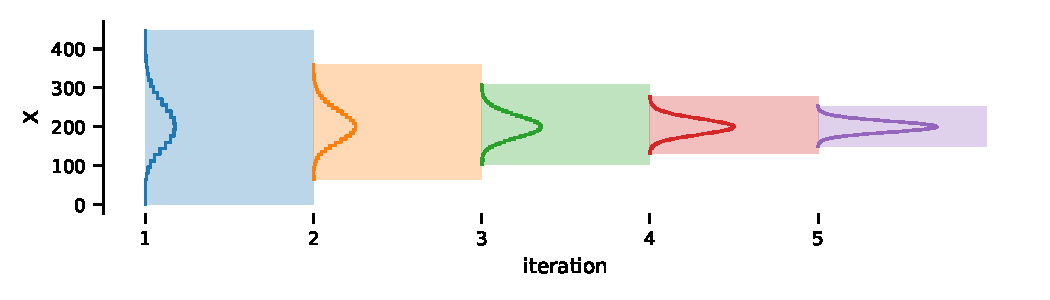
\includegraphics[width=8cm]{../gfx/bd_truncs.pdf}
    \end{figure}
    \end{exampleblock}
    \bottomcite{backenkohler2020analysis,backenkohler2021abstraction}
\end{frame}

\multipleframe
\foreach \n in {1,...,7}{
\begin{frame}{Stationary distribution}{Example}
    \begin{figure}
        \centering
        \includegraphics[width=11cm]{../gfx/eswitch_ref_\n.pdf}
        \vspace{1cm}
        \def\svgwidth{5cm}
        \input{../gfx/excl_switch_sketch.pdf_tex}
    \end{figure}
%\begin{gather*}
	%D + P_1 \xrightarrow{\beta} D.P_1\,,\quad
	%D.P1 \xrightarrow{\gamma_1} D + P_1  \,,\\
	%D + P_2 \xrightarrow{\beta} D.P_2 \,,\quad
	%D.P2 \xrightarrow{\gamma_2} D + P_2 \,,\\
	%D.P_1 \xrightarrow{\rho_1} D.P_1 + P_1\,, \quad
    %D.P_2 \xrightarrow{\rho_2} D.P_2 + P_2\,,\\
	%D \xrightarrow{\rho_1} D + P_1\,,\quad
	%D \xrightarrow{\rho_2} D + P_2\,,  \quad
	%P_1 \xrightarrow{\lambda}\varnothing  \,,\quad
    %P_2\xrightarrow{\lambda} \varnothing
%\end{gather*}
\bottomcite{backenkohler2021abstraction}
\end{frame}}
\restoreframe

\begin{frame}{Bridging problem}{Dynamical analysis under initial \emph{and} terminal constraints}
    \begin{figure}
        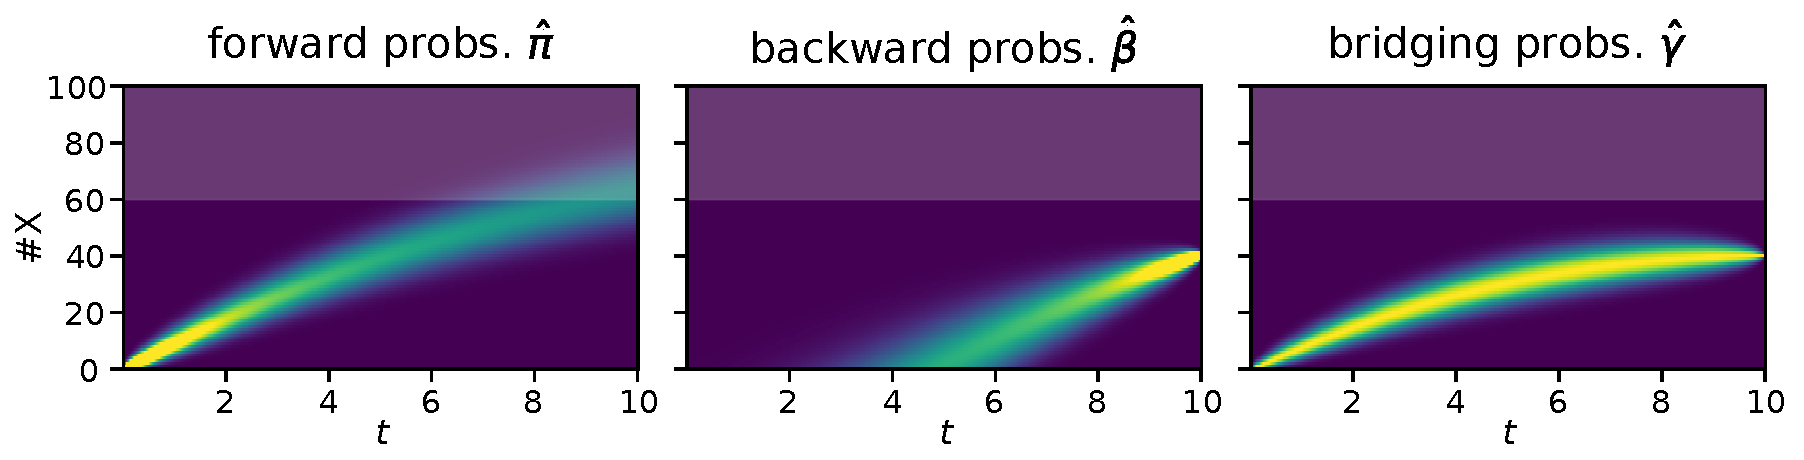
\includegraphics[width=7cm]{../gfx/bridging_bd.pdf}
    \end{figure}
    \begin{block}{Forward probabilities $\pi$}
        How the process evolves with time: $\Pr({X_t=x\mid X_0=0})$
    \end{block}
    \begin{block}{Backward probabilities $\beta$}
        Probability of ending up in a given state: $\Pr(X_T=40 \mid X_t = x)$
    \end{block}
    \begin{block}{Bridging probabilities $\gamma$}
        In between: $\Pr (X_t=x\mid X_0=0, X_T=40)$
    \end{block}
    \bottomcite{backenkohler2020analysis}
\end{frame}

\begin{frame}{Bridging problem}{Refinement}
    \begin{figure}
        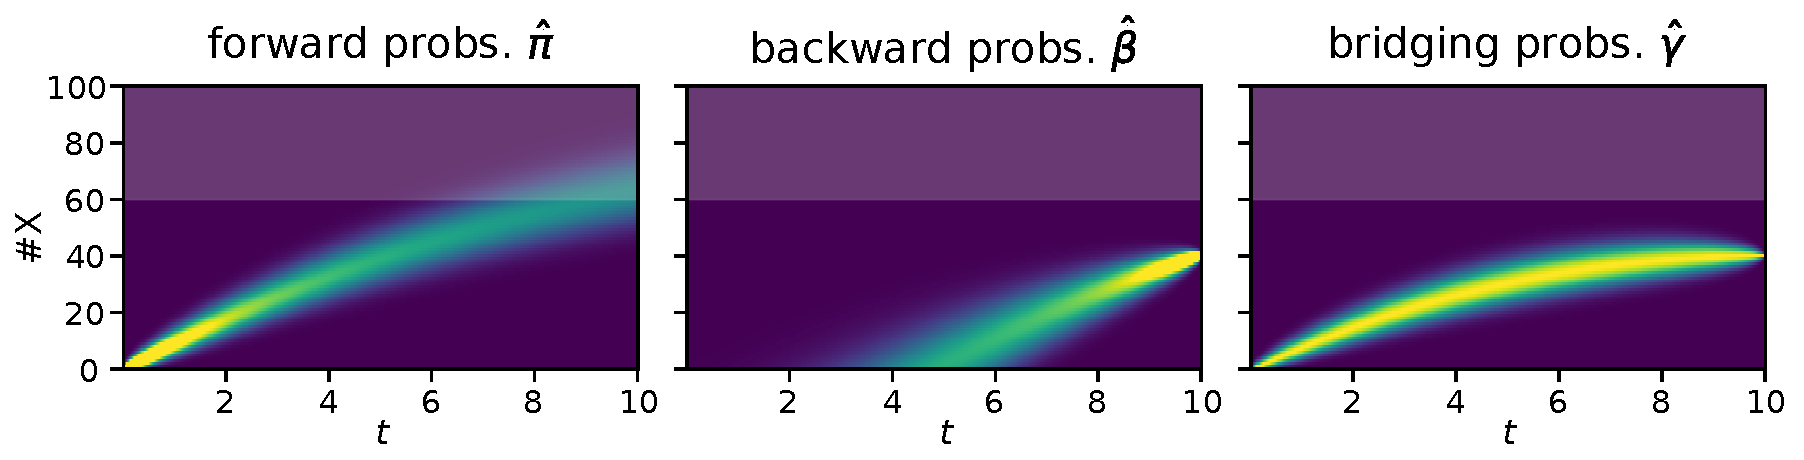
\includegraphics[width=7cm]{../gfx/bridging_bd.pdf}
    \end{figure}
    \begin{itemize}
        \item bridging distribution: 
            \[ 
            \gamma(x_i, t) = \pi(x_i, t)\beta(x_i, t)/\pi(x_g, T) \]
        \item record intermediary times
        \item remove or split based on $\hat{\gamma}(x_i, t)$
    \end{itemize}
    \begin{figure}
        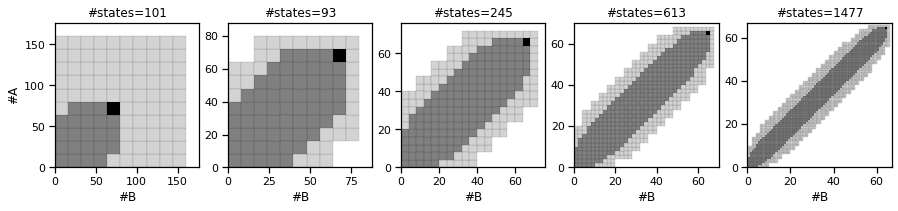
\includegraphics[width=10cm]{../gfx/refinement.png}
    \end{figure}

        %\transduration<0-16>{0.1}
        %\multiinclude[<+->][format=jpg, graphics={width=\textwidth}]{../gfx/bridge_anim/bridge}
    %\noindent\animategraphics[loop,width=\textwidth,autoplay]{10}{../gfx/bridge_anim/bridge-}{0}{99}
    \bottomcite{backenkohler2020analysis}
\end{frame}

\begin{frame}{Bridging problem}{Bayesian filtering in an SEIR model}
    \[ S+I \rightarrow E+I \qquad E\rightarrow I \qquad I\rightarrow R \]
    We know:
    \begin{itemize}
        \item initial state
        \item uncertain measurement of $I$ at $T=0.3$
    \end{itemize}
    We are interested in the posterior at $T$.
    \begin{columns}
        \begin{column}{.35\paperwidth}
            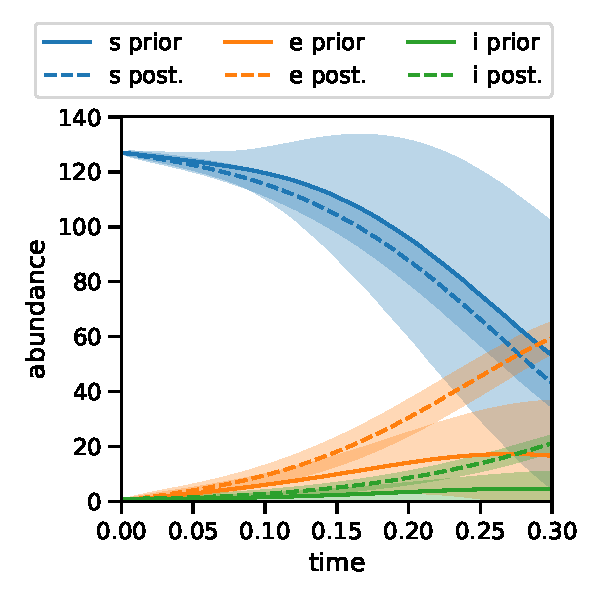
\includegraphics[width=\textwidth]{../gfx/seir_prior_posterior.pdf}
        \end{column}
        \begin{column}{.35\paperwidth}
            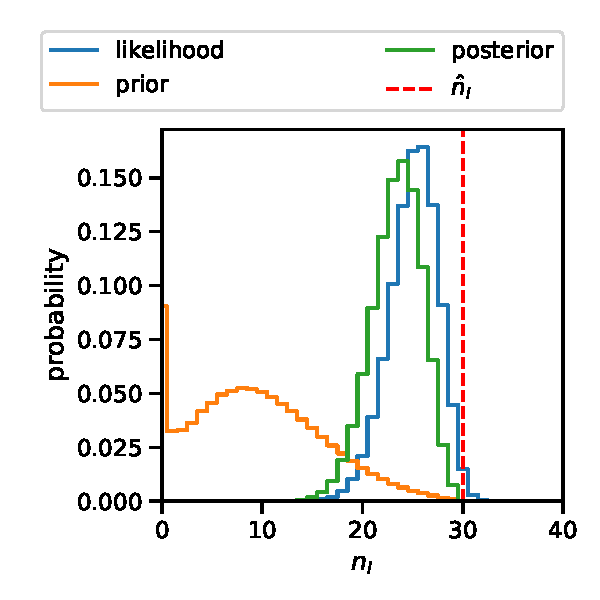
\includegraphics[width=\textwidth]{../gfx/posterior.pdf}
        \end{column}
        \begin{column}{.25\paperwidth}
            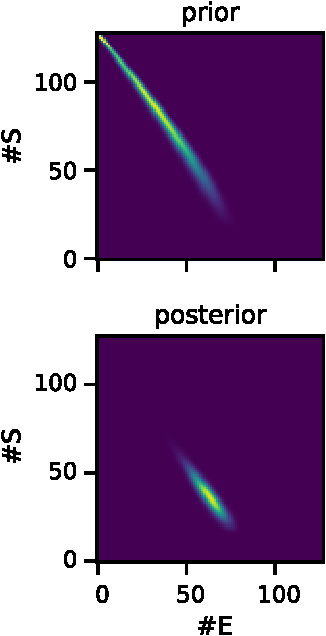
\includegraphics[width=.8\textwidth]{../gfx/prior_posterior_vert.pdf}
        \end{column}
    \end{columns}
    \bottomcite{backenkohler2020analysis}
\end{frame}
%\begin{frame}{Importance Sampling}
    
%\end{frame}

\section{Conclusion}
\begin{frame}{Contributions}
    \begin{columns}
        \begin{column}{.45\paperwidth}
            \begin{block}{Moment-based}
                \begin{itemize}
                    \item bounding of mean first-passage times \parencite{backenkohler2019bounding}
                        \begin{figure}
                            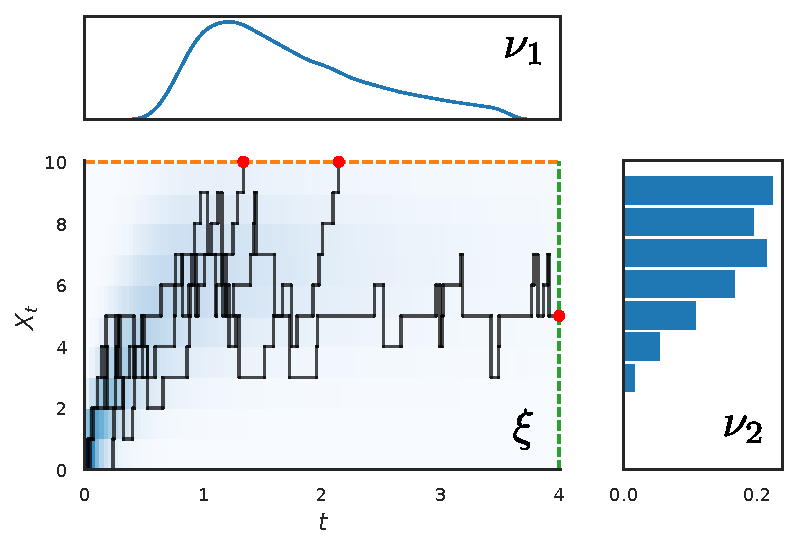
\includegraphics[width=.67\textwidth]{../gfx/decomp1.pdf}
                        \end{figure}
                    \item variance reduction for MC estimation \parencite{backenkohler2019control,backenkohler2021variance}
                        \begin{figure}
                            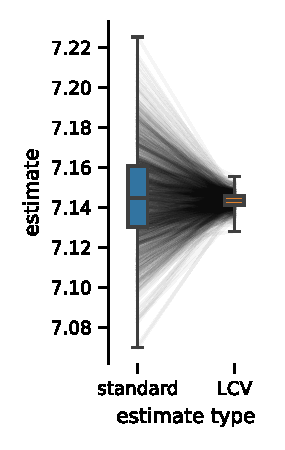
\includegraphics[width=.3\textwidth]{../gfx/adjustment_trans.pdf}
                        \end{figure}
                \end{itemize}
            \end{block}
        \end{column}
        \begin{column}{.45\paperwidth}
            \begin{block}{Aggregation \& refinement}
                \begin{itemize}
                    \item stationary distribution \parencite{backenkohler2021abstraction}
                        \begin{figure}
                            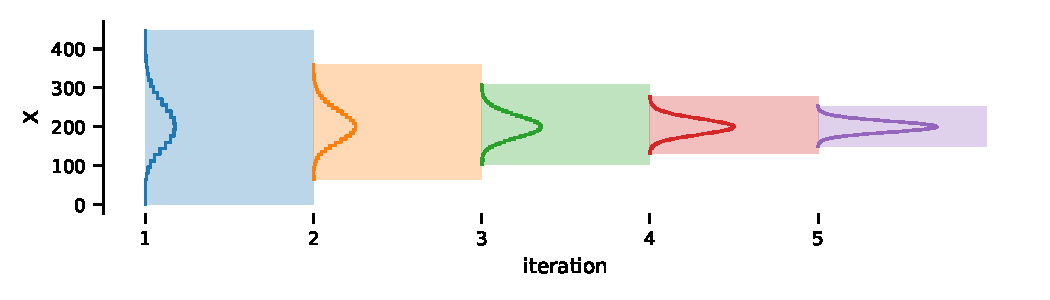
\includegraphics[width=4cm]{../gfx/bd_truncs.pdf}
                        \end{figure}
                    \item bridging distribution \parencite{backenkohler2020analysis}
                        \begin{figure}
                            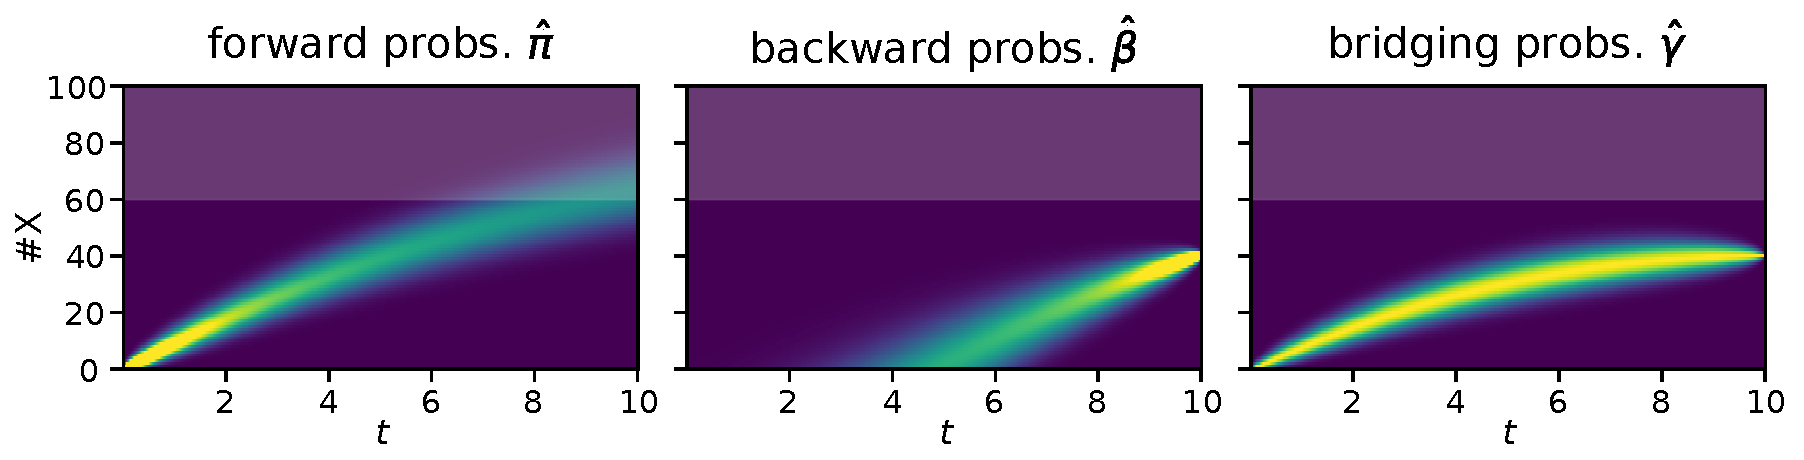
\includegraphics[width=4cm]{../gfx/bridging_bd.pdf}
                        \end{figure}
                    \item importance sampling
                        \begin{figure}
                            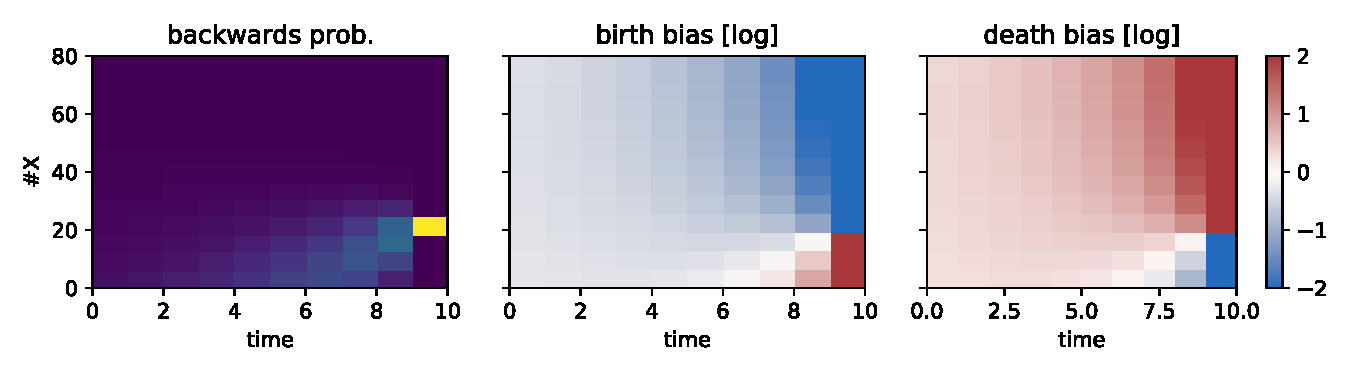
\includegraphics[width=5cm]{../gfx/biases.pdf}
                        \end{figure}
                \end{itemize}
            \end{block}
            \begin{block}{Augmented Lyapunov functions}
                local alteration of valid Lyapunov functions for tighter guarantees
            \end{block}
        \end{column}
    \end{columns}
    %\begin{itemize}
        %\item local augmentation of Foster-Lyapunov functions
        %\item state-space aggregation scheme
    %\end{itemize}
\end{frame}

\begin{frame}[allowframebreaks]
    \frametitle{References}
%        \bibliographystyle{amsalpha}
    \printbibliography
\end{frame}

\begin{frame}{Linear control variates}{Results}
    \begin{columns}
        \begin{column}{.05\paperwidth}\end{column}
        \begin{column}{.5\paperwidth}
            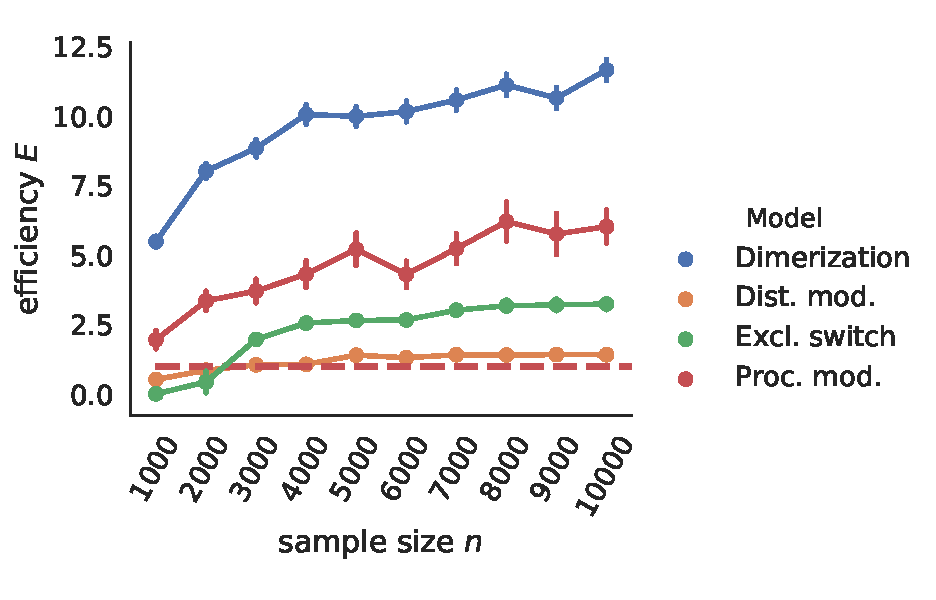
\includegraphics[width=\textwidth]{../gfx/sample_size.pdf}
                    \begin{columns}
                        \begin{column}{.6\textwidth}
                            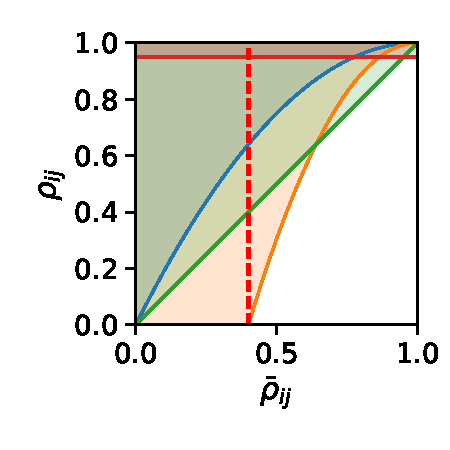
\includegraphics[width=\textwidth]{../gfx/decision_funcs.pdf}
                        \end{column}
                        \begin{column}{.39\textwidth}
                            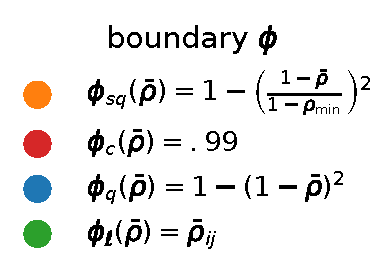
\includegraphics[width=\textwidth]{../gfx/legend_1.pdf}
                        \end{column}
                \end{columns}
        \end{column}
        \begin{column}{.1\paperwidth}\end{column}
        \begin{column}{.4\paperwidth}
            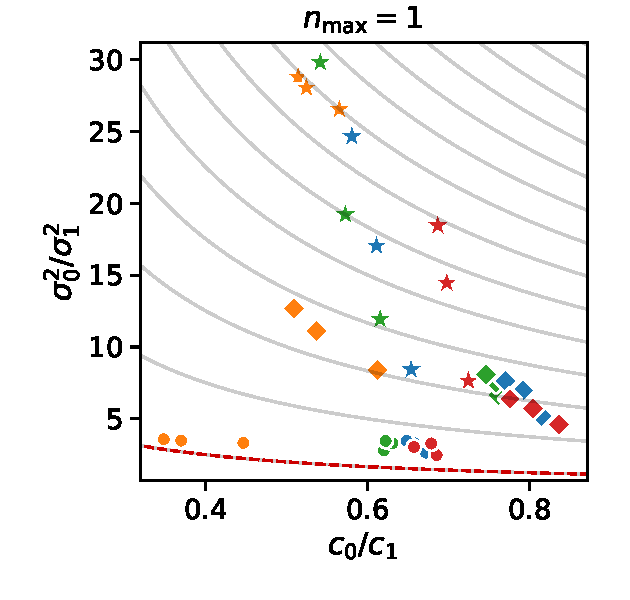
\includegraphics[width=4cm]{../gfx/eff_landscape_order1.pdf}\\
            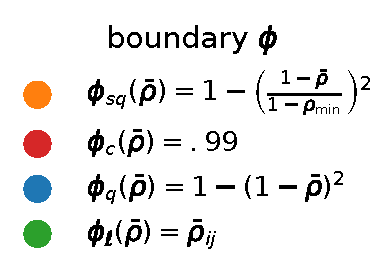
\includegraphics[width=27mm]{../gfx/legend_1.pdf}
            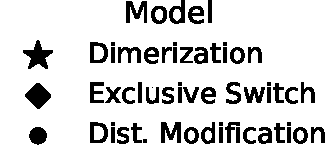
\includegraphics[width=27mm]{../gfx/legend_models.pdf}
        \end{column}
    \end{columns}
\end{frame}

\begin{frame}{Linear control variates}{Results}
    \begin{itemize}
        \item SMC can improve variance reduction
    \begin{figure}
        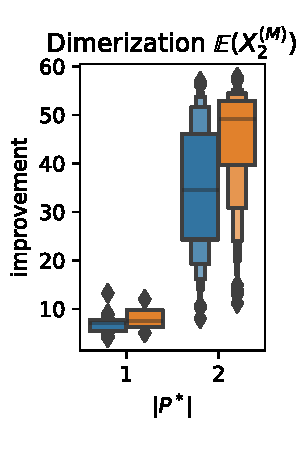
\includegraphics[scale=.4]{../gfx/dim_improvement_numcv.pdf}
        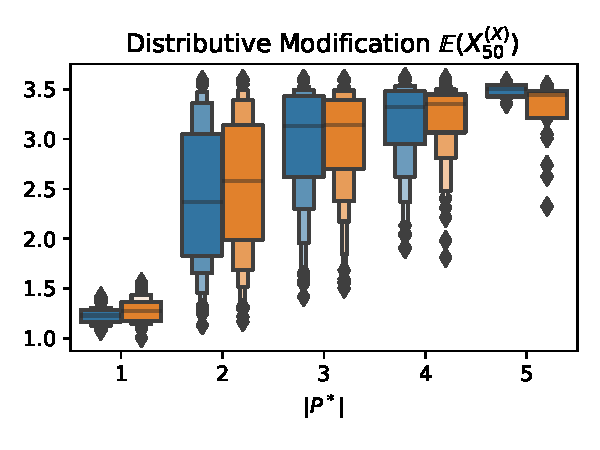
\includegraphics[scale=.4]{../gfx/dm_improvement_numcv.pdf}\\
        
\includegraphics[scale=.4]{../gfx/improvement_numcv_legend.pdf}
    \end{figure}
    \item less dependence on initial covariates
    \item more consistent performance
    \end{itemize}
\end{frame}


\iffalse
\begin{frame}{Foster-Lyapunov Functions}
\end{frame}

\begin{frame}{Local Augmentation of Foster-Lyapunov Functions}
\end{frame}

\begin{frame}{Control Variates in General}
\end{frame}

\begin{frame}{Control Variates Selection Algorithm 1}
\end{frame}

\begin{frame}{Control Variates Selection Algorithm 2}
\end{frame}

\begin{frame}{Semi-definite programming}
\end{frame}
\fi

\end{document}
